\documentclass[a4paper,12pt]{article}
% Gestion des images
\usepackage{graphicx}  % Permet l'insertion d'images
% Gestion des équations mathématiques avancées
\usepackage{amsmath}   % Pour les équations mathématiques avancées
% Gestion des légendes des graphiques et tableaux
\usepackage{caption}   % Pour les légendes des graphiques
% Liens hypertextes (références, URL cliquables)
\usepackage{hyperref}  % Pour les liens cliquables
% Gestion des sous-figures ou sous-tableaux
\usepackage{subcaption} % Pour les sous-figures
% Mise en page avancée (marges, taille de la page)
\usepackage{geometry}  % Pour personnaliser la mise en page
% Dessins vectoriels et graphiques (pour diagrammes et figures complexes)
\usepackage{tikz}      % Pour créer des graphiques avec TikZ
% Graphiques basés sur des données numériques
\usepackage{pgfplots} 
\usepackage{graphicx}
\usepackage{float} 
\title{TP d'évaluation : Modélisation et Analyse de Sensibilité d'un Forage}
\author{Mohamad SAMMAN}
\date{\today}

\begin{document}

\maketitle
\tableofcontents
\newpage
\section{Introduction}
Ce travail pratique vise à analyser un modèle de forage en utilisant une approche par simulation de Monte Carlo pour la propagation des incertitudes, ainsi qu'à réaliser une analyse de sensibilité des paramètres d'entrée. La fonction \texttt{borehole} est utilisée pour simuler le débit d'eau en fonction de 13 paramètres d'entrée. Nous allons appliquer plusieurs techniques statistiques pour analyser la propagation des incertitudes et la sensibilité du modèle.

\section{Mise en place du modèle et calculs initiaux}

Nous avons commencé par tester la fonction de forage \texttt{borehole()} en évaluant la sortie pour des valeurs minimales, moyennes et maximales des paramètres d'entrée. Les valeurs minimales et maximales ont été choisies directement à partir des plages spécifiées dans l'énoncé, tandis que la valeur moyenne de la loi lognormale a été calculée à partir des paramètres $ \mu = 7.71 $ et $ \sigma = 1.0056 $, en utilisant la formule :

\begin{equation}
\text{Moyenne de X} = \exp\left( \mu + \frac{\sigma^2}{2} \right)
\end{equation}

Nous avons ensuite évalué le débit pour les valeurs minimales, moyennes et maximales des paramètres.

\subsection{Résultats des évaluations}
Les résultats des évaluations du débit pour les valeurs minimales, moyennes et maximales sont présentés ci-dessous :
\begin{equation}
\text{Débit pour les valeurs minimales} = 6.308688 
\end{equation}
\begin{equation}
\text{Débit pour les valeurs moyennes} = 50.331380
\end{equation}
\begin{equation}
\text{Débit pour les valeurs maximales} = 150.145626
\end{equation}


\section{Propagation d’incertitudes par Monte Carlo}

\subsection{a) Moyenne, variance et histogramme}
Nous avons utilisé un échantillonnage Monte Carlo avec une taille d'échantillon de 1000 pour calculer la moyenne et la variance de la sortie. Un histogramme des valeurs de débit a également été tracé pour visualiser la distribution de la sortie.

Le graphique suivant montre l'histogramme des débits obtenus :
\begin{figure}[h!]
    \centering
    \includegraphics[width=0.7\textwidth]{histogramme.png}
    \caption{Histogramme des débits obtenus par échantillonnage Monte Carlo (1000 échantillons)}
\end{figure}

La moyenne et la variance calculées sont les suivantes :
\begin{equation}
\text{Moyenne} = 52.336676
\end{equation}
\begin{equation}
\text{Variance} = 678.4250205
\end{equation}

\subsection{b) Comparaison de la moyenne}
Nous avons comparé la moyenne de la sortie obtenue par Monte Carlo avec celle de la sortie évaluée à la moyenne des paramètres d'entrée. Les résultats sont les suivants :
\begin{equation}
\text{Moyenne Monte Carlo} = 52.336676
\end{equation}
\begin{equation}
\text{Moyenne de la sortie avec les entrées moyennes} = 50.331380
\end{equation}
La différence observée suggère que la fonction n'est pas strictement linéaire, ce qui est attendu pour ce type de modèle complexe.

\subsection{c) Quantile d'ordre 95\% et intervalle de confiance}
Nous avons calculé le quantile d'ordre 95\% de la sortie, ainsi qu'un intervalle de confiance à 95\% basé sur 1000 répétitions de l'échantillonnage Monte Carlo. Le quantile et l'intervalle de confiance sont les suivants :

\begin{equation}
\text{Quantile d'ordre 95\%} = 100.8539 
\end{equation}
\begin{equation}
\text{Intervalle de confiance à 95\%} = [15.71709, 114.63988]
\end{equation}

\subsection{d) Probabilité de dépassement du seuil de 250 m3/an}
Nous avons également calculé la probabilité que le débit dépasse 250 m³/an en augmentant progressivement la taille de l'échantillon. Nous sommes parti de $2\times10^6$ avec un pas de $2\times10^6$. On converge après 8 itération avec une taille d'échantillon de $1,8\times10^7$.
Le graphique suivant montre la convergence de la probabilité avec l'augmentation de la taille de l'échantillon :

\begin{figure}[h!]
    \centering
    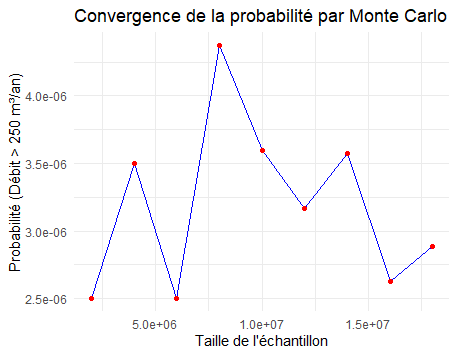
\includegraphics[width=0.7\textwidth]{conv.png}
    \caption{Convergence de la probabilité que le débit dépasse 250 m³/an en fonction de la taille de l'échantillon}
\end{figure}

\section{Analyse de sensibilité}

\subsection{a) Criblage avec la méthode de Morris}
Nous avons utilisé la méthode de Morris pour réaliser un criblage des paramètres d'entrée, en limitant le coût à moins de 100 évaluations de la fonction. Les résultats obtenus, présentés à la \autoref{morris}, permettent d'identifier les variables ayant un impact significatif sur la sortie: \(K_w\), \(r_w\), \(H_l\), \(H_0\), et \(L\). Avec \(K_w\)et \(r_w\) ayant un impact plus important que les trois autres. Nous verrons avec sobol qu'on aurait pu négliger \(H_l\), \(H_0\), et \(L\). 

Les variables présentant des valeurs élevées de $\mu^\star$ (moyenne des effets absolus) et de $\sigma$ (dispersion des effets) sont considérées comme influentes et devront être conservées pour les analyses ultérieures. En revanche, les variables avec des valeurs faibles de $\mu^\star$ et $\sigma$ sont considérées comme peu influentes ; elles peuvent donc être fixées à leur moyenne pour simplifier les analyses suivantes.
\begin{figure}[h!]
    \centering
    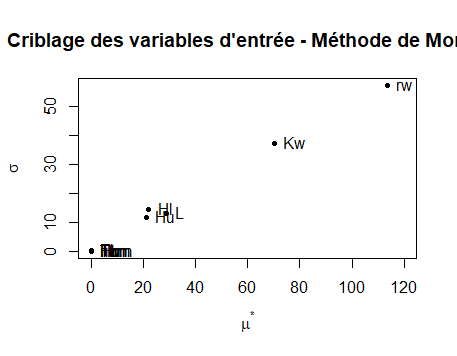
\includegraphics[width=0.7\textwidth]{morris.png}
    \caption{Indices de Sobol pour la fonction de forage}
    \label{morris}
\end{figure}
\\
\subsection{b) Indices basés sur la régression}
Nous pouvons observer le scatterplot \autoref{pairs}. Le comportement n'est pas linéaire (sauf potentiellement pour \(L\)). Chose qu'on savait déja puisque la moyenne des sorties n'est pas égale à la sortie des valeurs moyennes. Donc la régression que nous allons faire n'est forcément pertinente mais elle fait partie des question du TP :) 
\\
Les variables identifiées comme influentes par la méthode de Morris ont été utilisées pour ajuster un modèle de régression linéaire. Les indices de sensibilité calculés à partir de cette régression montrent l'importance relative de chaque variable \autoref{tab:SRC2}. Les variables influentes pour cette méthode sont \(H_l\), \(L\) et \(r_w\) alors que \(H_u\) et \(K_w\) ont une influence négligable sur la sortie. Ce qui n'est pas en accord avec ce qu'on trouve avec Monte-Carlo et sobol. Ceci n'est pas surprenant car le modèle n'est pas linéaire.
\begin{figure}[H]
    \centering
    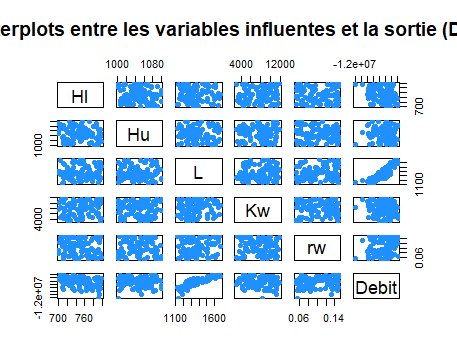
\includegraphics[width=0.7\textwidth]{pairs.png}
    \caption{Scatterplots entre les variables influentes et la sortie}
    \label{pairs}
\end{figure}
\begin{table}[H]
    \centering
    \begin{tabular}{|c|c|}
        \hline
        \textbf{Variable} & \textbf{Indice de sensibilité SRC²} \\
        \hline
        Hl & 0.420 \\
        Hu & 0.000006 \\
        L  & 0.102 \\
        Kw & 0.000022 \\
        rw & 0.478 \\
        \hline
    \end{tabular}
    \caption{Indices de sensibilité SRC² des variables influentes}
    \label{tab:SRC2}
\end{table} 

\subsection{c) Indices de Sobol}
Enfin, nous avons calculé les indices de Sobol pour toutes les variables en utilisant un échantillon adapté. Les résultats des indices de Sobol sont présentés \autoref{lol}, ce qui permet d'identifier les contributions des variables influentes: \(K_w\)et \(r_w\).

\begin{figure}[H]
    \centering
    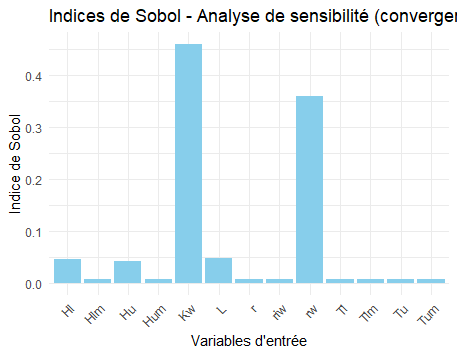
\includegraphics[width=0.7\textwidth]{sobolol.png}
    \caption{Indices de Sobol pour la fonction de forage}
    \label{lol}
\end{figure}

\section{Conclusion}
Ce travail a permis d'analyser un modèle de forage en utilisant la simulation de Monte Carlo pour évaluer la propagation des incertitudes et réaliser une analyse de sensibilité des paramètres d'entrée. Les résultats ont montré une non-linéarité du modèle, confirmée par les analyses de sensibilité. La méthode de Morris a mis en évidence les variables les plus influentes (\(K_w\), \(r_w\), \(H_l\), \(H_0\), \(L\)), tandis que les indices de Sobol ont révélé que la conductivité hydraulique du forage \(K_w\) et le rayon du forage \(r_w\) étaient les plus impactantes. La régression linéaire n’a pas permis d’identifier toutes les influences de manière satisfaisante, ce qui est cohérent avec la non-linéarité du modèle.
\end{document}
